The main objective was always the analysis of Telemetry. The best and most accurate option to study this component would have been to analyze it source code. Unluckily this isn't possible as the Windows kernel is not open source. However, it was still possible to reverse engineer the Windows kernel to understand how Telemetry works. 
Several files (dynamic libraries, executables, drivers) had to be reversed and analyzed. Nonetheless, there was one file that had the main focus: {\bfseries ntoskrnl.exe}. This binary holds the actual implementation of the Windows Kernel.

Following sections will depict different challenges and achievements faced during the analysis of this and the other binaries.



%%%%%%%%%%%%%%%%%%%%%%%%%%%%%%%%%%%%%%%%%%%%%%%%%%
%% Understanding how Telemetry makes use of ETW %%
%%%%%%%%%%%%%%%%%%%%%%%%%%%%%%%%%%%%%%%%%%%%%%%%%%

\section{Understanding how Telemetry makes use of ETW}\label{understanding_telemetry_etw}

When Windows OS boots, multiple sessions are created inside ETW. Among them there is one related to Telemetry: DiagTrack. As explained in \ref{ETW}, every session has "providers": those entities that actually provide information to the session. In order to understand how Telemetry works with ETW, it was important to learn about DiagTrack's session providers. To help us the following questions wanted to be answered:
\begin{enumerate}
\setlength\itemsep{0.05em}
\item Who are they?
\item Where are they?
\item What information are they logging?
\end{enumerate}

Windows allowed to query the list of providers registered to a particular session by executing the following powershell command: 

\begin{figure}[H]
  \begin{lstlisting}
    Get-EtwTraceProvider | where {$_.SessionName -match 
    "<SESSION_NAME>"}
  \end{lstlisting} 
  \caption[]{Powershell command to list ETW providers registered against a particular session. }
  \label{fig:powershell_cmd}
\end{figure}
For each provider registered to the queried session, the following information is outputted:
\begin{itemize}
  \setlength\itemsep{0.05em}
  \item GUID
  \item TO\_CHECK
  \item TO\_CHECK
\end{itemize}

With this list the question {\bfseries Who are they?} seems to be answered. However, two questions are still missing to answer.

At this point and idea came up: To answer {\bfseries Where are they running?} and {\bfseries What are they logging?} it could be useful to hook into the exact moment when any of those providers are going to write to the DiagTrack's session. 
In other words, it could be useful to set a breakpoint in the function that performs the write to the DiagTrack's session. Once the breakpoint is hit, the following information could be extracted:

\begin{enumerate}
\setlength\itemsep{0.05em}
\item The piece of code that triggered the write (by inspecting the function's call stack). In other words, identify who is writing. 
\item The actual content of the log being written.
\end{enumerate} 

That was when debugging (\ref{debugging}) came into play. Analyzing the symbols exposed by the ntoskrnl binary, the function {\bfseries EtwWrite} was found. This function seemed to be one in charge of carrying out the writes of providers inside sessions. Nonetheless, it wasn't worth to set a breakpoint at this function as every provider of the system (not necessarily related to DiagTrack) could use it. 
It was necessary to find a way of only detecting the writes performed by DiagTrack's providers. 

Let's recall the powershell command (\ref{fig:powershell_cmd}). This command will return you information for each registered provider. Part of that information was the GUID. 

The objective was to filter writes only from providers that were registered against the DiagTrack Session. To do so the idea was to set a conditional breakpoint inside function {\bfseries EtwWrite} and try to check if the GUID provided was of interest.

Unfortunately, this strategy had one minor issue. The function ({\bfseries EtwWrite}) had five parameters and none of them would show directly the GUID:

\begin{figure}[H]
  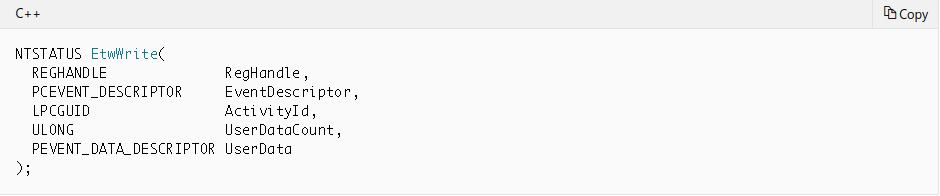
\includegraphics[width=\linewidth]{images/etw_write_docu.png}
  \caption[]{Documentation for EtwWrite function \footnote{https://docs.microsoft.com/en-us/windows-hardware/drivers/ddi/content/wdm/nf-wdm-etwwrite}. }
  \label{fig:etw_write_docu}
\end{figure}

The first parameter is the registration handler. This object is returned once the provider executed the registration ({\bfseries EtwRegister)} successfully.
However, taking a look to {\bfseries EtwRegister} it is possible to observe that it receives the GUID as parameter:
\begin{figure}[H]
  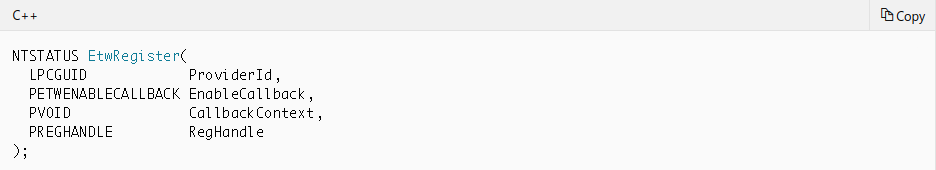
\includegraphics[width=\linewidth]{images/etw_register_docu.png}
  \caption[]{Documentation for EtwRegister function \footnote{https://docs.microsoft.com/en-us/windows-hardware/drivers/ddi/content/wdm/nf-wdm-etwregister}.}
  \label{fig:etw_register_docu}
\end{figure}

This finding basically meant that having only one breakpoint in {\bfseries EtwWrite} wasn't going to be enough as information from {\bfseries EtwRegister} was also needed.

In other words, to understand if the write was being done by a provider registered against the DiagTrack session it was necessary to: 
\begin{enumerate}
\setlength\itemsep{0.05em}
    \item Extract the whole list of providers registered against the DiagTrack session.
    \item Intercept all the {\bfseries EtwRegister} executions and check if the GUID being used was inside the list.
    \item If it was, save the handler. 
    \item Intercept all the {\bfseries EtwWrite} executions and check if the handler being used is one of the stored handlers.
    \item If it was, the provider that is writing, is attached to the DiagTrack session.
\end{enumerate}

Even though this strategy seemed to be theoretically promising, it was necessary to understand how to actually carry out each of these steps. Further sections will depict this process.





%%%%%%%%%%%%%%%%%%%%%%%%%%%%%%%%%%%%
%% Reversing registration process %%
%%%%%%%%%%%%%%%%%%%%%%%%%%%%%%%%%%%%

\subsection{Reversing registration process}\label{reversing_registration_process}
As mentioned in section \ref{ETW}, whenever a provider wants to register itself against a particular session it has to call the function {\bfseries EtwRegister}. Because of this, the first step was to analyze the behavior of this function using {\bfseries IDA}(\ref{IDA}). 

As can be seen in figure \ref{fig:etwRegister_code}, the only interesting action being performed by {\bfseries EtwRegister} was a call to another function named {\bfseries EtwpRegisterProvider}. 

\begin{centering}
\begin{figure}[H]
  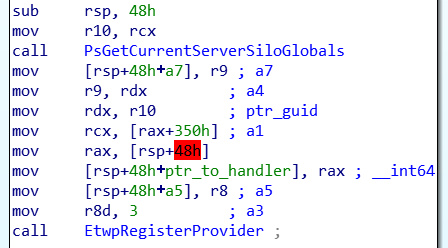
\includegraphics[width=12cm]{images/etwRegister_code.png}
  \caption[]{Dissasembly of ETWRegister function}
  \label{fig:etwRegister_code}
\end{figure}
\end{centering}

A quick analysis of the latter function showed that it was the function holding the actual implementation of the registration process. However, due to the lack of documentation, it was necessary to understand in a more in-depth way what was actually happening inside it.

Following chapters will present a detailed description of reversing (partially, only the interesting parts for this research) {\bfseries EtwpRegisterProvider}. 
To make it easier, it will be divided in different parts:

\begin{itemize}
  \setlength\itemsep{0.05em}
  \item 1. Understanding the layout of the function
  \item 2. Check if a GUID for this provider already exists.
  \item 3. If not, create a new one
  \item 4. Return the handler.
\end{itemize}

\begin{figure}[H]
\begin{lstlisting}
// 1. Understanding the layout of the function 
signed __int64 __fastcall EtwpRegisterProvider(__int64 a1, _QWORD *a2, int a3, void (__fastcall *a4)(ULONG_PTR, __int64, __int128 *,__int64), __int64 a5, __int64 a6, __int64 *a7){

[..]

// 2. Check if a GUID for this provider already exists.
ptr_guid_entry = (char *)EtwpFindGuidEntryByGuid(etw_silo, ptr_guid, 0);

// 3. If not, create a new one
if ( ptr_guid_entry || (ptr_guid_entry = EtwpAddGuidEntry(ptr_etw_silo_cpy2, ptr_guid_cpy, 0)) != 0i64 )
{
  v15 = __readgsqword(0x188u);
  --*(_WORD *)(v15 + 484)
  
  [..]

  // 4. Return the handler.
  v35 = EtwpAddKmRegEntry((ULONG_PTR)ptr_guid_entry, v10, (__int64)v9, a5, (__int64)&ptr_handler);
  v20 = v35;

  [..]

}
return v20;
\end{lstlisting}
\caption[]{EtwpRegisterProvider snippet .}
\label{fig:etwpRegisterProvider_listing}
\end{figure}












  %%%%%%%%%%%%%%%%%%%%%%%%%%%%%%%%%%%%%%%%%%%%%%
  %% Understanding the layout of the function %%
  %%%%%%%%%%%%%%%%%%%%%%%%%%%%%%%%%%%%%%%%%%%%%%

  \subsubsection{\bfseries{1. Understanding the layout of the function}}
  {\bfseries EtwpRegisterProvider} received seven parameters:
  \begin{verbatim}
  signed __int64 __fastcall EtwpRegisterProvider(__int64 a1, _QWORD *a2,
        int a3, void (__fastcall *a4)(ULONG_PTR, __int64, __int128 *,
        __int64), __int64 a5, __int64 a6, __int64 *a7)
  \end{verbatim}

  Usually when performing reverse engineering it is not necessary to understand every tiny detail but only the key points that are important to meet the proposed goals. This wasn't the exception. 

  The main focus here was not to understand how the registration process fully worked but just to get an idea of it plus get to know the relation between GUID and registration handler.

  After analyzing  {\bfseries EtwpRegisterProvider} it was possible to conclude that:
  \begin{enumerate}
\setlength\itemsep{0.05em}
  \item {\bfseries a1}: Is the pointer to a structure.
  \item {\bfseries a2}: Is the pointer to the GUID structure. 
  \item {\bfseries a7}: Is the address where the pointer to the registration handler will be placed (can be think as "function output").
  \end{enumerate}

  What is this {\bfseries a1} structure?
  The figure \ref{fig:etwRegister_code} shows that before calling {\bfseries EtwpRegisterProvider}, the function {\bfseries PsGetCurrentServerSiloGlobals} is invoked. This latter one returns a pointer to a structure $S$ of type {\bfseries \_ESERVERSILO\_GLOBALS}. 

  \begin{centering}
  \begin{figure}[H]
    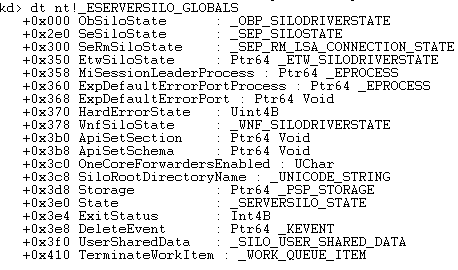
\includegraphics[width=12cm]{images/ESILOGLOBALS_structure.png}
    \caption[]{\_ESERVERSILO\_GLOBALS structure layout ($S$).}
    \label{fig:eserversilo_globals_structure}
  \end{figure}
  \end{centering}

  However, the first parameter provided to {\bfseries EtwpRegisterProvider} is not the pointer to $S$ but is the pointer to another structure $S_2$ of type {\bfseries \_ETW\_SILODRIVERSTATE}. which is part of $S$, more precisely, it is situated at offset 0x350. 

  \begin{centering}
  \begin{figure}[H]
    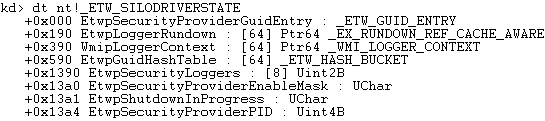
\includegraphics[width=12cm]{images/ETW_SILODRIVERSTATE_structure.png}
    \caption[]{\_ETW\_SILODRIVERSTATE structure layout ($S_2$).}
    \label{fig:etwsilodriverstate_structure}
  \end{figure}
  \end{centering}

  With this information it was possible to conclude that {\bfseries a1} will point to a global structure holding configurations, settings and information in general directly related with the {\bfseries ETW} framework. {\bfseries a2} and {\bfseries a7} will hold pointers to a GUID and to a place were a registration handler will be stored afterwards. 

  With the information gathered from this analysis was enough to move forward.\\


 Once inside the $EtwpRegisterProvider$ function, after performing some sanity checks, it tries to get the guid entry related to the GUID provided. If it doesn't exist, it will create one. 
  
  \begin{centering}
  \begin{figure}[H]
    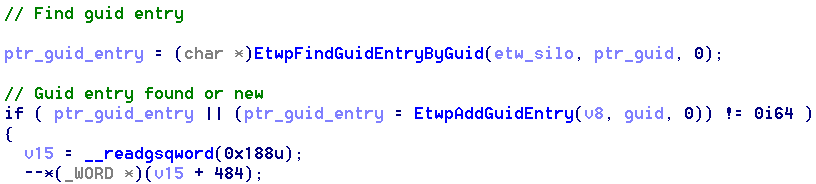
\includegraphics[width=15cm]{images/etwpregisterProvider.png}
    \caption[]{First lines of EtwpRegisterProvider}
    \label{fig:etwpregisterProvider}
  \end{figure}
  \end{centering}


  %%%%%%%%%%%%%%%%%%%%%%%%%%%%%%%%%%%%%%%%%%%%%%%%%%%%
  %% Check if GUID for this provider already exists %%
  %%%%%%%%%%%%%%%%%%%%%%%%%%%%%%%%%%%%%%%%%%%%%%%%%%%%

  \subsubsection{\bfseries{2. Check if GUID for this provider already exists}}
 
  In this part, the focus will be on understanding how the process of recovering the already existing "GUID entry" works.

  The action of recovering is performed by a particular function called {\bfseries EtwpFindGuidEntryByGuid}:

  \begin{verbatim}
  ptr_guid_entry = (char *)EtwpFindGuidEntryByGuid(etw_silo, ptr_guid, 0);
  \end{verbatim}

  As can be inferred from the previous line, two important parameters are provided: the {\bfseries ETWSILODRIVERSTATE}(a1) structure $S$ and the pointer to the GUID $ptr\_guid$.

  \begin{centering}
  \begin{figure}[H]
    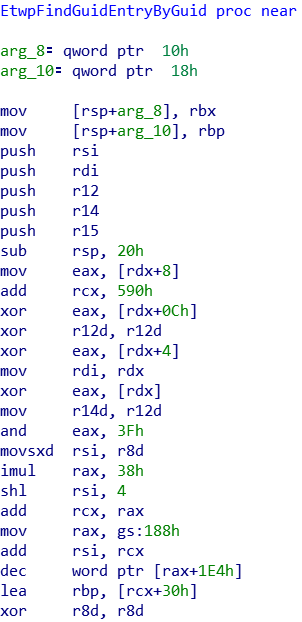
\includegraphics[width=6cm]{images/etwpfindguidguidentrybyguid1.png}
    \caption[]{First basic block of EtwpFindGuidEntryByGuid.}
    \label{fig:EtwpFindGuidEntryByGuid}
  \end{figure}
  \end{centering}

  Figure \ref{fig:EtwpFindGuidEntryByGuid} depicts how the function gets the guid entry related to the provider (if it exists): $rcx$ holds the pointer to $S$ and $rdx$ holds $ptr\_guid$. Let's analyze this function deeper.

  The first highlight is the $add$ function which stores in $rcx$ the pointer to the structure stored at the offset $0x590$ of $S$. Going back to the structure layout of $S$ (figure \ref{fig:etwsilodriverstate_structure}), it can be appreciated that at the offset $0x590$, the structure $EtwpGuidHashTable$ of type $\_ETW\_HASH\_BUCKET[64]$ is present. Figure \ref{fig:etwhashbucketlayout} depicts its layout.

  Just before the $add$ function, $eax$ is filled with the content of the address $rdx+8$. $rdx$ held the $ptr\_guid$, meaning that $eax$ will have the third group of 4 bytes inside of the guid structure. Why the third? Because the offset was 8. Why 4 bytes? Because the register $eax$ (32 bits) was used.

  In the following lines, the value of $eax$ is being constantly modified by xoring it successively with the different group of 4 bytes that compose the guid structure\footnote{Sometimes the structures weren't documented at all. Sometimes they were, but was not possible to find it until some kind of clue pointing to it was found.  So far the layout of the structure pointed by $ptr\_guid$ was unknown, however from this function it was possible to conclude that the structure had a size of 16 bytes.}. After performing these successive xor operations, a boolean and is applied against $eax$ (result of xoring) using a mask of $0x3f$. This mask will set all $eax$ bits to 0 with the exception of the last 6 that will remain having its actual value. The reason to do this is because $2^6 = 64$. In other words, this mask is making the xoring result fit into the range of a valid bucket index. Afterwards, multiplies the result against $0x38$ (size of $\_ETW\_HASH\_BUCKET$ structure). Finally, the value of $rax$($eax$) is added to $rcx$ which had the pointer to the $EtwpGuidHashTable$ structure. 

  Writing the aforementioned function in a pseudo-code style ($ptr$ is a short version of "pointer"): 
  \begin{verbatim}
  xor_guid_parts = ptr_guid[0] ^ ptr_guid[1] ^ ptr_guid[2] ^ ptr_guid[3]
  ptr_hash_table = ptr_S + 0x590
  ptr_bucket = ptr_hash_table + 0x38 * ((xor_guid_parts) & 0x3F) 
  \end{verbatim}

  Therefore, $ptr\_bucket$ is basically a pointer to a particular bucket inside the $EtwpGuidHashTable$ calculated based on the GUID of the provider\footnote{There was also an additional value involved in the calculation of the bucket. However, in this particular context, the value wasn't taken into account as it was always 0. }. 
  Once this value is obtained, a "look up" inside the structure is carried out in the following way:

  \begin{centering}
  \begin{figure}[H]
    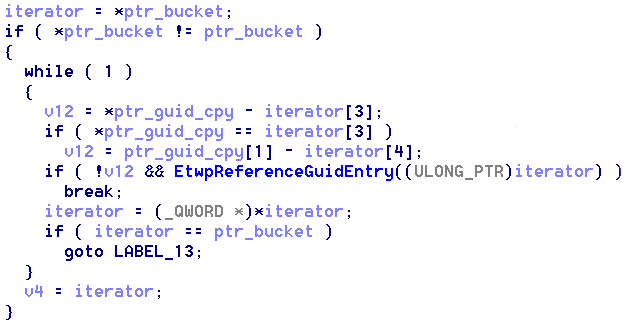
\includegraphics[width=12cm]{images/etwpfindguidentrybyguid_while.png}
    \caption[]{Part of EtwpFindGuidEntryByGuid function extracted using IDA Hex-Rays plugin.}
    \label{fig:EtwpFindGuidEntryByGuid_while}
  \end{figure}
  \end{centering}

  \begin{centering}
  \begin{figure}[H]
    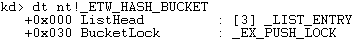
\includegraphics[width=10cm]{images/_etw_hash_bucket_structure.png}
    \caption[]{$\_ETW\_HASH\_BUCKET$ structure layout.}
    \label{fig:etwhashbucketlayout}
  \end{figure}
  \end{centering}

  At first an iterator is built. This iterator will point initially to the Flink of the first list entry\footnote{https://docs.microsoft.com/en-us/windows/desktop/api/ntdef/ns-ntdef-\_list\_entry} of the bucket (figure \ref{fig:etwhashbucketlayout}). The right-after "if" will capture the special case were the list is empty. In that particular case, the whole cycle will be skipped and the {\bfseries LABEL\_13} (routine to exit, which isn't displayed in the figure) will be executed. It's worth to mention that this routine executes a return statement with the value of the variable $v4$ (which is initially defined as 0).

  If the list is not empty, the first operation which is carried out is a subtraction between the first quadword of the GUID and a value of $iterator[3]$. Due to the variable $iterator$ is defined as a 8-bytes pointer, $iterator[3]$ will point to the offset $0x18$ of the structure stored inside the Flink. In the case that both values are equal, the second comparison (between the second quadword of the GUID and the $iteartor[4]$) is carried out. 

  At this point some things can be concluded:
  \begin{itemize}
  \setlength\itemsep{0.05em}
  \item The cycle is iterating a double-linked-list which holds a particular structure $T$.
  \item $T$ has the GUID of the provider stored at offset $0x18$
  \item Again, seems that the GUID is 16 bytes long.
  \item From the function name it can concluded that $T$ is a structure that represents the GUID entry.
  \end{itemize}

  Moving forward with the code analysis, if some of the comparisons failed, the iterator changes its values to the next one in the list. Before continuing, it ensures that the cycle is not finished by checking if the actual value of the iterator is the same one used as the starting point. If they are equal, the exit routine is executed meaning that the return value will be 0.

  If both comparisons are equal (the GUID of the provider and the one stored in $T$ are the same), a function called $EtwpReferenceGuidEntry$ with the current value of the iterator as parameter, is called. After this execution, the cycle is finished by the break statement. However, before executing the exit routine, the value of $v4$ is filled up with the value of the $iterator$, meaning that the return value will be pointer to the guid entry related to the GUID of the provider. The $EtwpReferenceGuidEntry$ function just made some security checks not relevant for this task. \\

  Therefore, to summarize, it is possible to say that:\\
  {\bfseries The function $EtwpFindGuidEntryByGuid$ looks for a particular structure (most probably called guid entry), which is stored inside a double-linked-list of a bucket inside the $EtwpGuidHashTable$ of the $\_ETW\_SILODRIVERSTATE$, based on doing some mathematical operations with the GUID of the provider.}\\


  After finishing with this analysis, the documentation of the guid entry structure was found: 

  \begin{centering}
    \begin{figure}[H]
      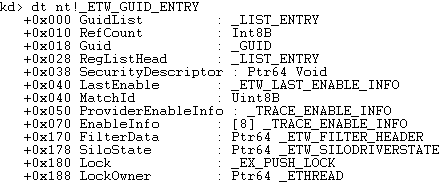
\includegraphics[width=12cm]{images/etwguidentrylayout.png}
      \caption[]{$\_ETW\_GUID\_ENTRY$ structure.}
      \label{fig:etwguidentrylayout}
    \end{figure}
  \end{centering}

  \begin{centering}
    \begin{figure}[H]
      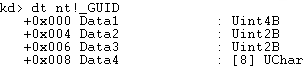
\includegraphics[width=8cm]{images/etwguidlayout.png}
      \caption[]{$\_ETW\_GUID$ structure.}
      \label{fig:guidlayout}
    \end{figure}
  \end{centering}
  
  Luckily, all the previous guesses made, were correct:
  \begin{itemize}
  \setlength\itemsep{0.05em}
    \item The guid entry (now $\_ETW\_GUID\_ENTRY$) had the GUID of at offset $0x18$ (figure \ref{fig:etwguidentrylayout})
    \item The GUID was a structure of 16 bytes long (figure \ref{fig:guidlayout})
  \end{itemize}



%%%%%%%%%%%%%%%%%%%%%%%%%%%%%%%%%%
%% IF NOT FOUND CREATE A NEW ONE%%
%%%%%%%%%%%%%%%%%%%%%%%%%%%%%%%%%%

\subsubsection{\bfseries{3. If not found, create a new one}}
Previous section detailed how was the process to find an already existing guid entry based on the GUID of the provider. This one will explain the process of creating a new guid entry.

From figure \ref{fig:etwpregisterProvider} can be observed that the function in charge of this part is the function $EtwpAddGuidEntry$:

\begin{verbatim}
  ptr_guid_entry = EtwpAddGuidEntry(ptr_etw_silo_cpy2, ptr_guid_cpy, 0)
\end{verbatim}

As can be inferred from the previous line, two important parameters were provided: the pointer to the \_ETW\_SILODRIVERSTATE structure (for simplicity will be called $ptr\_etw\_silo$ instead of $ptr\_etw\_silo\_cpy2$) and the pointer to the GUID (for simplicity will be called $ptr\_guid$ instead of $ptr\_guid\_cpy$).

One of the first lines of $EtwpAddGuidEntry$, calls another function named $EtwpAllocGuidEntry$. As it can be quickly inferred from the name, it basically allocates certain amount of memory inside the heap to be used by the guid entry afterwards and returns the pointer to it. The allocation part happens in the first basic block of $EtwpAllocGuidEntry$:

  \begin{centering}
    \begin{figure}[H]
      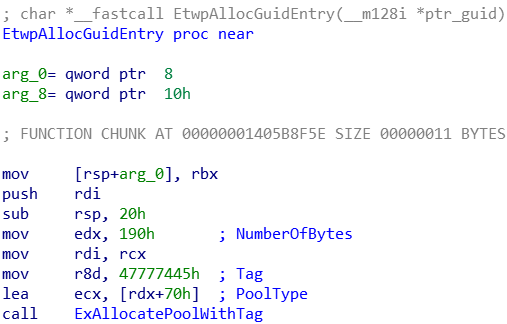
\includegraphics[width=12cm]{images/etwpallocguidentry.png}
      \caption[]{$EtwpAllocGuidEntry$ allocation.}
      \label{fig:etwallocguidentry}
    \end{figure}
  \end{centering}

As can be observed in figure \ref{fig:etwallocguidentry} the Windows function $ExAllocatePoolWithTag$\footnote{Documentation: https://docs.microsoft.com/en-us/windows-hardware/drivers/ddi/content/wdm/nf-wdm-exallocatepoolwithtag} is called with the following parameters:
\begin{itemize}
  \setlength\itemsep{0.05em}
  \item {\bfseries PoolType}: 0x200 ({\bfseries NonPagedPoolNx}). This value indicates that the system memory allocated will be nonpageable and not executable\footnote{Documentation: https://docs.microsoft.com/en-us/windows-hardware/drivers/ddi/content/wdm/ne-wdm-\_pool\_type}.
  \item {\bfseries NumberOfBytes}: 0x190. This value is the size of the structure $\_ETW\_GUID\_ENTRY$ (figure \ref{fig:etwguidentrylayout}).
  \item {\bfseries Tag}: "0x47777445". According the documentation just a four character long to be used as the pool tag. Due to it is specified in reverse order: 0x45747747 $\rightarrow$ "EtwG".
\end{itemize}

Therefore, as it was thought, $EtwpAllocGuidEntry$ allocs the necessary memory for holding the $\_ETW\_GUID\_ENTRY$ structure and returns a heap pointer to it. \\


The remaining code of $EtwpAddGuidEntry$ is devoted to populate and adjust some parts of related structures. Some key points about it: 
\begin{itemize}
  \setlength\itemsep{0.05em}
\item A guid entry related to this GUID is looked up inside the guid entries double-linked list using the same technique as the one used in $EtwpFindGuidEntryByGuid$. If a structure is found, the pointer is freed.
\item Only three parts of the $\_ETW\_GUID\_ENTRY$ structure are populated at this point:
  \begin{enumerate}
\setlength\itemsep{0.05em}
  \item The pointer to the previous guid entry in the double-linked list (offset 0x0)
  \item The pointer to the following guid entry in the double-linked list (offset 0x8)
  \item The pointer to the SILO STATE (offset 0x178)
  \end{enumerate}
\end{itemize}


To summarize, once $EtwpAllocGuidEntry$ is executed, the pointer to heap memory holding the $\_ETW\_GUID\_ENTRY$ structure is returned. The next step is insert this entry into $EtwpGuidHashTable$. To perform that action, first it looks for the correct place to insert it as depicted previously.




%%%%%%%%%%%%%%%%%%%%%%%%%%%%%%%%%%
%%     RETURN THE HANDLER       %%
%%%%%%%%%%%%%%%%%%%%%%%%%%%%%%%%%%

\subsubsection{\bfseries{4. Return the handler}}

Going back to what the figure \ref{fig:etw_register_docu} states, the 4th parameter of $EtwRegister$ it's something of type $PREGHANDLE$. Although it isn't very clear, this parameter is the output of the function (usually called "out" type of parameter). Furthermore, as it was mentioned previously the real registration logic is implemented by $EtwpRegisterProvider$ therefore the output of $EtwRegister$ is none other than the output of $EtwpRegisterProvider$.\\


Despite the fact the provider's GUID existed previously or not, at this point it exist a pointer to a $\_ETW\_GUID\_ENTRY$ structure holding its data and already inside the main structures of ETW. 
Once the code achieved this point, the next step is basically get the handler.

Just right after the pointer to the $\_ETW\_GUID\_ENTRY$ is found, the function $EtwpAddKmRegEntry$ is called:
\begin{verbatim}
__int64 __usercall EtwpAddKmRegEntry(ULONG_PTR a1, int a2, __int64 a3,
__int64 a4, __int64 a5)
\end{verbatim}

where :
\begin{enumerate}
\setlength\itemsep{0.05em}
  \item {\bfseries a1}: Is the pointer to $\_ETW\_GUID\_ENTRY$, called $ptr\_guid$. 
  \item {\bfseries a5}: Is the memory address provided by $EtwWrite$ (and afterwards by $EtwpRegisterProvider$) where the handler should be placed. 
\end{enumerate}
The remaining parameters are not interesting for the sake of our research.\\

Once inside $EtwpAddKmRegEntry$, the first important lines were:

\begin{centering}
  \begin{figure}[H]
    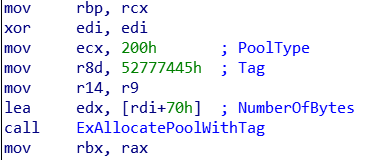
\includegraphics[width=8cm]{images/etwpaddkm_reserve_heap_for_handler.png}
    \caption[]{$EtwpAddKmRegEntry$ allocation.}
    \label{fig:etwpaddkm_allocate_handler}
  \end{figure}
\end{centering}

As can be inferred from \ref{fig:etwallocguidentry}, this is also an allocation in the heap: 

\begin{itemize}
  \setlength\itemsep{0.05em}
  \item {\bfseries PoolType}: 0x200 ({\bfseries NonPagedPoolNx}).
  \item {\bfseries NumberOfBytes}: 0x70. As depicted in the image, $rdi$ is first set to 0. 
  \item {\bfseries Tag}: "0x52777445". According the documentation just a four character long to be used as the pool tag. Due to it is specified in reverse order: 0x45747752 $\rightarrow$ "EtwR".
\end{itemize}


The analysis of the following lines of $EtwpAddKmRegEntry$ showed how the aforementioned reserved space (structure) was being filled. While debugging this function the following line excelled from the rest:
\begin{lstlisting}
mov     [rbx+20h], rbp
\end{lstlisting}

The reason to excelled was that, at that point, $rbp$ held the pointer to the GUID entry. Meaning that this structure, potentially the registration handler structure, has the pointer to the GUID entry at offset 0x20. After finish filling the rest, the pointer to the structure is returned.

Going back to \ref{fig:etwpRegisterProvider_listing}, it can be appreciated that the output of $EtwpAddKmRegEntry$ is the output of $EtwpRegisterProvider$ too. Which confirmed that this was the registration handler structure.

After finishing with this analysis, the documentation of the registration handler structure was found:

\begin{centering}
  \begin{figure}[H]
    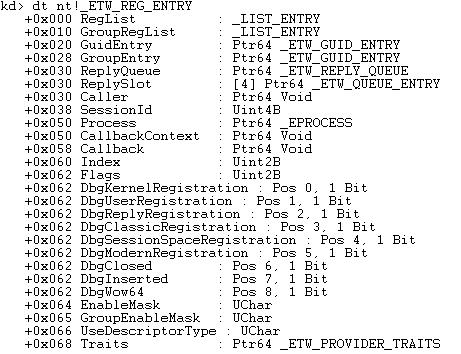
\includegraphics[width=12cm]{images/etw_reg_entry.png}
    \caption[]{$\_ETW\_REG\_ENTRY$ structure .}
    \label{fig:regentrylayout}
  \end{figure}
\end{centering}



%%%%%%%%%%%%%%%%%%%%%%%%%%%%%%%%%%%%%%%%%%%%%%%%%%%%
%%%%  First steps into catching writes from providers  %%%%%%
%%%%%%%%%%%%%%%%%%%%%%%%%%%%%%%%%%%%%%%%%%%%%%%%%%%%


\section{First steps into catching writes from providers}
In section \ref{understanding_telemetry_etw} an idea on how to answer two important questions was presented: Hook in the exact moment when providers write to DiagTrack's session. However the idea would have been unfeasible without the analysis performed in section \ref{reversing_registration_process}.

At this point it is possible to detect if a particular provider is writing by knowing just its GUID. However it was important to understand to which session this provider was writing. For an initial analysis a mix between automatic and manual analysis was performed. A breakpoint in the function {\bfseries EtwWrite} was set using the following Windbg(\ref{Windbg}) script:
\begin{lstlisting}
bp nt!EtwWrite ".printf \"Handler: %N\\n\",@rcx"
\end{lstlisting}

This script just printed the address of provider's registration handle that is making a write (@$rcx$ holds the first parameter of the function according to Windows x64 calling convention). Once the handler's address was obtained it was possible to get the GUID as well. Comparing the GUID with the output of the powershell command {\bfseries Get-EtwTraceProvider } (without filters) threw an interesting result: Most of the time a provider with E02A841C-75A3-4FA7-AFC8-AE09CF9B7F23 as GUID was the one writing. This provider wasn't related with DiagTrack at all. 

The following step was to filter out this provider: 
\begin{lstlisting}
bp nt!EtwWrite ".if (@rcx != ffffda839f0c2c50){.printf \"Handler: %N\\n\",@rcx;gc;}.else{gc;} "
\end{lstlisting}

Unfortunately, providers which weren't related to DiagTrack neither flooded the output of the script. Clearly, this wasn't a good path. 

With the goal of pursuing interesting results, the function was changed by another one called {\bfseries EtwWriteTransfer}:.

\begin{lstlisting}
bp nt!EtwWriteTransfer ".if (@rcx != ffffda839f0c2c50){.printf \"Handler: %N\\n\",@rcx;gc;}.else{gc;}"
\end{lstlisting}

This time, a new provider attached to DiagTrack with GUID E9EAF418-0C07-464C-AD14-A7F353349A00 appeared. In order to get some more information, the script was updated once more to get the Call Stack of the provider's process:
\begin{lstlisting}
bp nt!EtwWriteTransfer ".if (@rcx == FFFFDA83A036F0D0){.printf \"Handler: %N\\n\",@rcx;kc;gc;}.else{gc;} "
 
 Call Site
00 nt!EtwWriteTransfer
01 nt!TlgWrite
02 nt!CmpInitHiveFromFile
03 nt!CmpCmdHiveOpen
04 nt!CmLoadAppKey
05 nt!CmLoadDifferencingKey
06 nt!NtLoadKeyEx
07 nt!KiSystemServiceCopyEnd
08 ntdll!NtLoadKeyEx
09 0x0
\end{lstlisting}

At this point, the only way so far to detect when providers related to DiagTrack were writing consisted in two steps: 
\begin{enumerate}
\setlength\itemsep{0.05em}
\item Hook in the ETW write function call.
\item Check if the provider is attached to DiagTrack based on its GUID and the output of the powershell command.
\end{enumerate}

However, even if it was a DiagTrack's related provider the one writing, it is not enough to ensure that it is currently writing to DiagTrack's session as providers could be attached to several sessions.

This quick result made two new questions to be raised
\begin{enumerate}
\setlength\itemsep{0.05em}
  \item 1. Is {\bfseries EtwWrite} the only write function used? (clearly no!)
  \item 2. How can we sure that a provider is actually writing to DiagTrack's session
\end{enumerate}

Further and deeper analysis was needed.

\subsection{\bfseries{ETW functions to write}}

A quick analysis of the symbols and cross references of the {\bfseries ntoskrnl.exe} binary showed that there were actually a "group of functions" that could be used to perform writes within the ETW framework:

\begin{centering}
  \begin{figure}[H]
    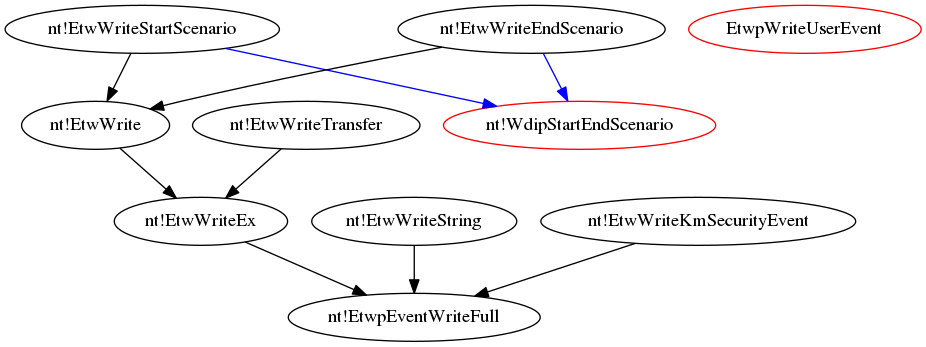
\includegraphics[width=15cm]{images/write_functions.png}
    \caption[]{Group of ETW Write functions.}
    \label{fig:etw_write_group_functions}
  \end{figure}
\end{centering}

As can be appreciated in figure \ref{fig:etw_write_group_functions} all functions end up calling  either {\bfseries nt!EtwpEventWriteFull} or {\bfseries nt!EtwpWriteUserEvent} or {\bfseries nt!WdispStartEndScenario}. After extensive analysis logging all actions and which functions were executed it was possible to detect that the function {\bfseries nt!WdispStartEndScenario} was never called under the context of interest of this research and therefore it was possible to discard it from further analysis. 


\subsection{\bfseries{Ensuring providers write to DiagTrack session}}
The previous idea of only analyzing writes from providers that were returned by the powershell command had, at least, three problems:

\begin{enumerate}
\setlength\itemsep{0.05em}
  \item The output of the powershell command returns the providers that are registered in a particular session at a given time $t$. If a provider registers, writes and unregisters itself from the session in a given time $t_2$ with $t_2 \neq t$, that write won't be took into consideration.
  \item Even if the provider is registered against DiagTrack's session, this doesn't ensure the provider is currently writing to it.
  \item It relied too much on manual analysis.
\end{enumerate}

With these problems in mind new ideas started to appear. In particular there was one that made the difference: What if it's possible to relate the handler that it's used at the moment of writing, with the session where the provider going to write, somehow. If that's possible, the first two problems would be solved. The third one could be solved as only one breakpoint at the writing function will be enough to make the full analysis. In order to find this relationship, an analysis of different structures related to ETW had to be performed.

Following section will detail the process of analyzing this structures together with its results.


\subsubsection{\bfseries Inspecting ETW structures}
So far it happened a lot that ETW structures were the key to overcome different obstacles. The first structure analyzed was $\_ETW\_REG\_ENTRY$ (figure \ref{fig:regentrylayout}) as it would have been the most direct and easier way to relate session and provider. Unfortunately, none of its components was helpful.

The next structure analyzed was $\_WMI\_LOGGER\_CONTEXT$. This structure seemed to be represent an ETW session. Due to the size of this structure only the necessary and representative offsets are depicted: 

\begin{figure}[H]
  \begin{lstlisting}
   +0x000 LoggerId         : Uint4B
   +0x004 BufferSize       : Uint4B
   +0x008 MaximumEventSize : Uint4B
   +0x00c LoggerMode       : Uint4B
   +0x010 AcceptNewEvents  : Int4B
   [...]
   +0x070 ProviderBinaryList : _LIST_ENTRY
   +0x080 BatchedBufferList : Ptr64 _WMI_BUFFER_HEADER
   +0x080 CurrentBuffer    : _EX_FAST_REF
   +0x088 LoggerName       : _UNICODE_STRING
   +0x098 LogFileName      : _UNICODE_STRING
   +0x0a8 LogFilePattern   : _UNICODE_STRING
   +0x0b8 NewLogFileName   : _UNICODE_STRING
   [...]
   +0x428 LastBufferSwitchTime : _LARGE_INTEGER
   +0x430 BufferWriteDuration : _LARGE_INTEGER
   +0x438 BufferCompressDuration : _LARGE_INTEGER
  \end{lstlisting} 
  \caption[]{$\_WMI\_LOGGER\_CONTEXT$ structure.}
  \label{fig:wmi_logger_context}
\end{figure}

Each session created inside the ETW framework will be represented by one of this structures. At offset $0x70$ there is an attribute called {\bfseries ProviderBinaryList}. After a quick analysis this attribute seemed to held all providers registered against the session in the format of a double linked list. In order to confirm that theory, the process of attaching new providers to an existing session was analyzed. 

The function $nt!EtwpAddProviderToSession$ seemed to be the one creating these links. However due to several reasons (lot of unknown new functions, hard to reverse and more) the analysis was cancelled. Besides the mentioned reasons there was one that was actually the one that made the preivous analysis to got cancelled: The finding of a new and promising structure. 

\subsubsection{\bfseries New structure: Trace enable info}

Among all structures related to the ETW there was one called $\_TRACE\_ENABLE\_INFO$:

\begin{centering}
  \begin{figure}[H]
    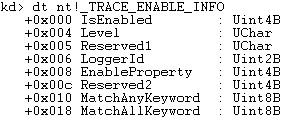
\includegraphics[width=9cm]{images/trace_enable_info.png}
    \caption[]{Trace Enable Info structure.}
    \label{fig:trace_enable_info}
  \end{figure}
\end{centering}

This structure seemed to contain the relation between a session and the provider (bingo!). This structure was found by analysing $\_ETW\_GUID\_ENTRY$ and how it was used when executing writing functions. As can be seen in figure \ref{fig:etwguidentrylayout}, at offset $0x50$ and $0x70$ there are structures of type $\_TRACE\_ENABLE\_INFO$.


the first one... is.. 
the second one is an array... 


nside the handler structure, we found one (seems to be special) of this guys and afterwards an array of 8 of them. Doing some empiric (TODO: Find this in the code) tests, I realize that if a provider is enabled for a session, then the "special" one will have the activated field in 1, but nothing in the loggerid field. Seems that this "special" is only for telling that the provider is enabled, but if you want more information about it you should go to each bucket of the array. Experience tell that if the "special" has the field activated in 1, there must be at least one bucket in the array with information about a session. There, you'll find, in the loggerid field, so this is our link to the session!.

\subsubsection{\bfseries asdassds}










%%%%%%%%%%%%%%%%%%%%%%%%%%%%%%%%%%
%%      To be written           %%
%%%%%%%%%%%%%%%%%%%%%%%%%%%%%%%%%%

\newpage
{\huge 1. We couldn't ensure that the data was being written was actually going to the DiagTrack session .}

\section{When and how providers are registered}
\section{How writes are carried out}
\section{Relation between ETW session and ETW providers}
\section{Identifying the buffers}
\section{Provider GUID vs Group Provider GUID}
\section{Checking correctness of logged events}
\section{Automatization of event logging}
\section{Service isolation}
\section{Triggers}
\section{searching for new triggers} YARA
\section{Difference among configuration levels of telemtry}
\section{Analysis of sent data over the channel to Microsfot backend services}
